\documentclass[dvipdfmx]{beamer}
\usepackage{tutorial}

\title{計算機実験(L6) --- 最適化問題}
\date{2016/06/15}

\begin{document}

\begin{frame}
  \titlepage
  \tableofcontents
\end{frame}

\section{最適化問題}

\begin{frame}[t,fragile]{最適化問題}
  \begin{itemize}
    %\setlength{\itemsep}{1em}
  \item 目的関数$f(x)$の最小値(あるいは最大値)とその場所を求めたい
    \begin{itemize}
    \item 連続最適化問題
    \item 離散最適化(組み合わせ最適化)問題 $\Leftarrow$ 難しい
    \end{itemize}
  \item 真の(大局的な)最小値(最大値)を求めるのは難しい
  \item 一般的には極値を求めることしかできない
  \item 多次元では極小を囲い込むことができない
  \item 導関数を使う方法: ニュートン法、最急降下法、共役勾配法、準ニュートン法
  \item 使わない方法: 囲い込み法、Nelder-Meadの滑降シンプレックス法、シミュレーテッド・アニーリング
  \end{itemize}
\end{frame}

\section{囲い込み法}

\begin{frame}[t,fragile]{囲い込み法(一次元の最適化)}
  \begin{itemize}
    \setlength{\itemsep}{1em}
  \item $f(a) > f(b) < f(c)$を満たす3点の組$a < b < c$の領域を狭めていく
  \item $[a,b]$、$[b,c]$の広い方(例えば後者)を$b$から見て
    $0.382:0.618$ (黄金比)に内分する点を$x$とする
    \begin{itemize}
    \item $f(b) > f(x)$の場合: $[b,c]$を新しい領域にとる
    \item $f(b) < f(x)$の場合: $[a,x]$を新しい領域にとる
    \end{itemize}
  \item もともとの$b$が$[a,c]$を$0.382:0.618$に内分する点だった場合、
    新しい領域の幅は、どちらの場合も0.618
  \item 最初の比率が黄金比からずれていたとしても、黄金比に収束
  \end{itemize}
\end{frame}

\begin{frame}[t,fragile]{最初の囲い込み}
  \begin{itemize}
    \setlength{\itemsep}{1em}
  \item 1点を選び、適当な$\Delta x$を取る
  \item 左右に$\Delta x$動かしてみて、関数値が小さくなる方へ動く
  \item どちらに進んでも関数値が大きくなる場合には、囲い込み完了
  \item 小さくなった場合、その方向へ再び増えるまで$\Delta x$を倍々に増やしながら進む
  \item 最後の3点で極小値を囲い込むことができる
  \end{itemize}
\end{frame}

\begin{frame}[t,fragile]{極小値をとる$x$の精度}
  \begin{itemize}
    \setlength{\itemsep}{1em}
  \item 実数の有効桁数を16桁($\epsilon \approx 10^{-16}$)とする(倍精度)
  \item 真の極小($x_0$)のまわりでテイラー展開
    \[
    f(x) \approx f(x_0) + \frac{1}{2} f''(x_0) (x-x_0)^2
    \]
  \item $f''(x_0) / f(x_0)$が$O(1)$だとすると
    \[
    |x-x_0| \sim \sqrt{\epsilon} \sim 10^{-8}
    \]
    以下になると、第二項の第一項に対する比が$\epsilon$よりも小さくなる
  \item それ以上領域を狭めても、関数値は変化しない
  \end{itemize}
\end{frame}

\section{ニュートン法}

\begin{frame}[t,fragile]{ニュートン法}
\end{frame}

\begin{frame}[t,fragile]{準ニュートン法}
\end{frame}

\section{最急降下法と共役勾配法}

\begin{frame}[t,fragile]{最急降下法(steepest-descent)}
  \begin{itemize}
    %\setlength{\itemsep}{1em}
  \item 関数の微分の情報を使う
  \item 現在の点$\bf x$における勾配を計算
    \[
    -\nabla f|_i = -\frac{\partial f}{\partial x_i}
    \]
  \item 坂を下る方向にそって、一次元最適化
  \item 動いた先の勾配の方向でさらに最適化を繰り返す
  \item 関数値は単調減少 $\Rightarrow$ 極小値に収束
  \end{itemize}
\end{frame}

\begin{frame}[t,fragile]{細長い谷の場合}
  \vspace*{1em}
  \hspace*{1em}\resizebox{1\textwidth}{!}{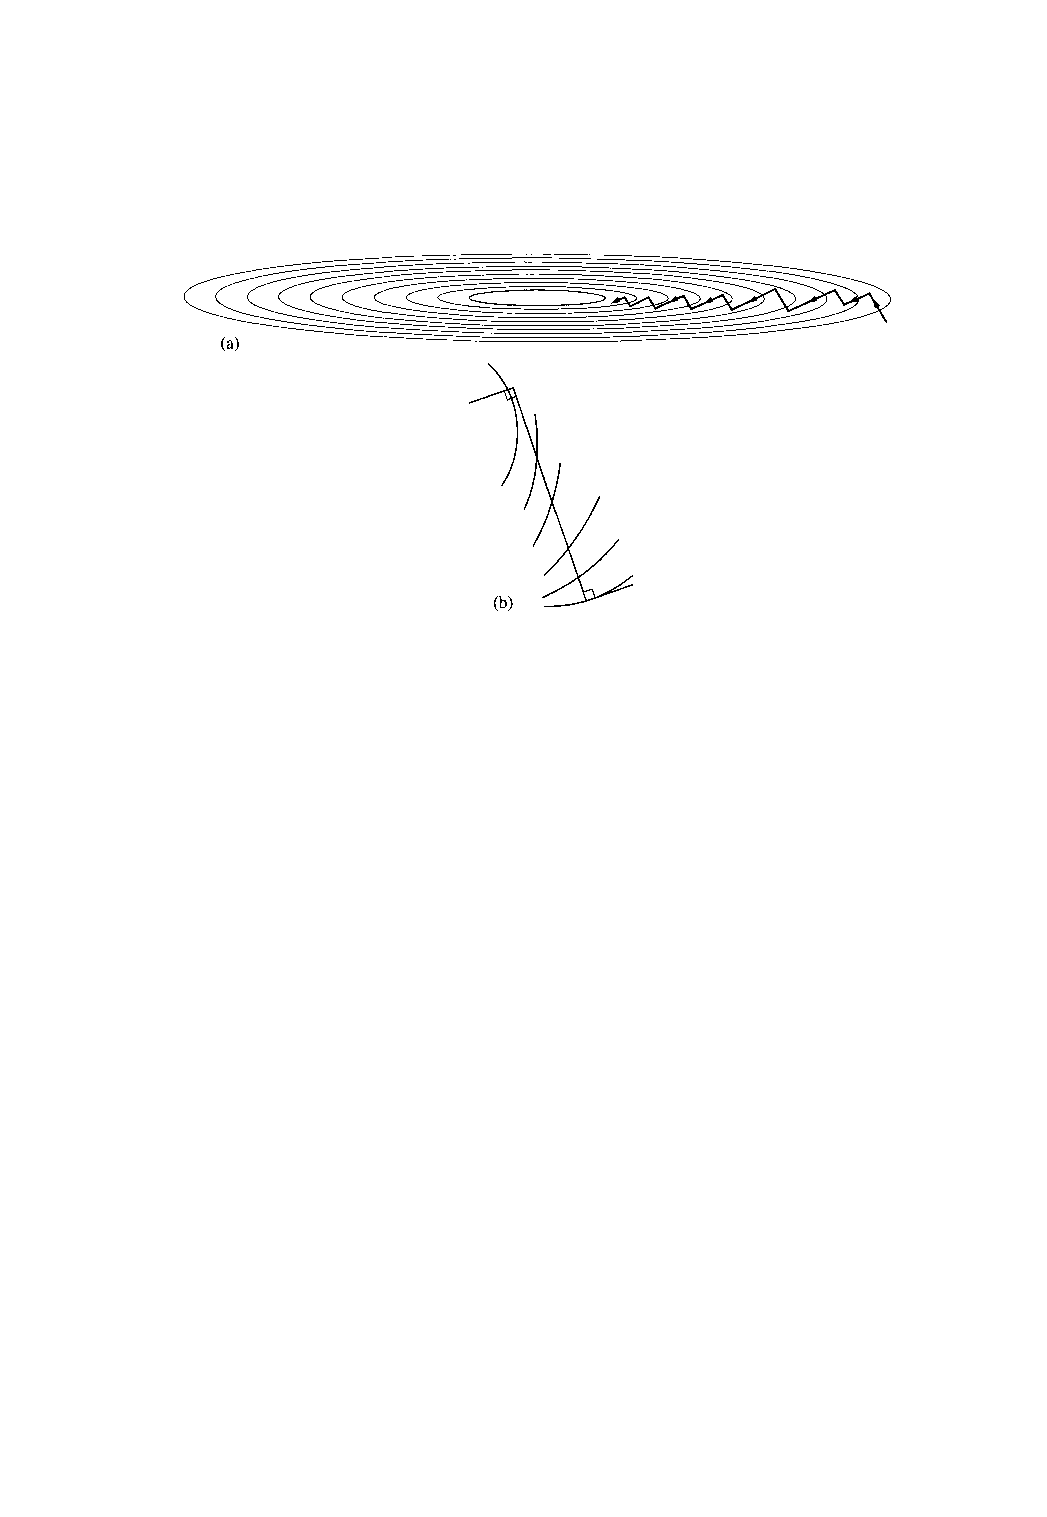
\includegraphics{image/steepest-descent.pdf}}

  \vspace*{-2em}
  \hspace*{20em}{\footnotesize(Press et al 1988)}
\end{frame}

\begin{frame}[t,fragile]{共役勾配法(conjugate-gradient)}
  \begin{itemize}
    \setlength{\itemsep}{1em}
  \item 関数がある点のまわりで
    \[
    f({\bf x}) \approx c - {\bf b}^T {\bf x} + \frac{1}{2} {\bf x}^T A {\bf x}
    \]
    と近似できるとする
  \item この時、${\bf x}$における勾配は、連立方程式$A{\bf x}={\bf b}$の「残差」の形で書ける
    \[
    -\nabla f = {\bf b} - A {\bf x}
    \]
  \item 新しい勾配方向ではなく、それまでとは「共役な方向」に進みたい
  \end{itemize}
\end{frame}

\begin{frame}[t,fragile]{「共役な方向」とは}
  \begin{itemize}
    \setlength{\itemsep}{1em}
  \item あるベクトル${\bf p}$にそった一次元の最適化が完了したとする
    \begin{itemize}
    \item その点における${\bf p}$方向の勾配は零。すなわち${\bf p}^T (\nabla f)=0$
    \item ${\bf p}$方向の勾配の値を変化させないようにしたい
  \end{itemize}
  \item 次に、${\bf q}$にそって、${\bf x}+\epsilon {\bf q}$と移動すると
    \[
      \delta(\nabla f) = A \times (\epsilon {\bf q}) \sim A {\bf q}
      \]
      これが${\bf p}$に垂直であり続けるためには
    \[
      {\bf p}^T A {\bf q} = 0
      \]
    \item この関係が成り立つ時、${\bf p}$と${\bf q}$は「互いに共役」という
  \end{itemize}
\end{frame}

\begin{frame}[t,fragile]{共役勾配法(Conjugate-gradient)}
  \begin{itemize}
    \setlength{\itemsep}{1em}
  \item 初期条件と漸化式
    \begin{align*}
      {\bf p}_0 &= {\bf r}_0 = {\bf b} - A {\bf x}_0 \\
      {\bf x}_{n+1} &= {\bf x}_n + \alpha_n {\bf p}_n \\
      {\bf r}_{n+1} &= {\bf r}_n - \alpha_n A {\bf p}_n = {\bf b} - A {\bf x}_{n+1} \\
      {\bf p}_{n+1} &= {\bf r}_{n+1} + \beta_n {\bf p}_n \\
      \alpha_n &= \frac{{\bf r}_n^T {\bf r}_n}{{\bf p}_n^T A {\bf p}_n} \ \ \
      \beta_n = \frac{{\bf r}_{n+1}^T {\bf r}_{n+1}}{{\bf r}_n^T {\bf r}_n}
    \end{align*}
  \item このように作ると、全ての$i>j \ge 1$について、自動的に
    \[
      {\bf p}_i^T A {\bf p}_j = 0 \ \ \ {\bf r}_i^T {\bf r}_j = 0
      \]
  \end{itemize}
\end{frame}

\begin{frame}[t,fragile]{共役勾配法(Conjugate-gradient)}
  \begin{itemize}
    \setlength{\itemsep}{1em}
  \item 残差は互いに直交 $\Rightarrow$ $N$回反復すると残差は零 (完全な二次形式の場合)
  \item 残差は負の勾配で表される $\Rightarrow$ $A$を知らなくても${\bf r}_i$は計算可
  \item 実際には、数値誤差により、共役性・直交性がくずれる
  \item また、完全な二次形式ではない
  \item しかし、最急降下法と比較すると圧倒的に速く収束
  \end{itemize}
\end{frame}

\begin{frame}[t,fragile]{逆反復法による固有ベクトルの計算}
  \begin{itemize}
    \setlength{\itemsep}{1em}
  \item $f(x)$の極小解は、連立一次方程式$A{\bf x} = {\bf b}$の解
    \begin{itemize}
    \item 連立方程式を解くのに共役勾配法を利用可
    \item 行列ベクトル積だけで計算できるので、$A$が疎行列の時、特に有効
    \end{itemize}
  \item 逆反復法
    \begin{itemize}
    \item 近似固有値を$\mu$とするとき、行列$(A - \mu I)^{-1}$を考えると、固有ベクトルは$A$と同じ、固有値は$(\lambda-\mu)^{-1}$。
    \item $\mu$が十分に正確であれば、$(\lambda-\mu)^{-1}$は絶対値最大の固有値。行列$(A - \mu I)^{-1}$を適当な初期ベクトルにかけ続けると$\lambda$に対応する固有ベクトルに収束(c.f. べき乗法)
    \item 実際には$(A-\mu I) {\bf x}' = {\bf x}$という連立方程式を繰り返し解く
    \end{itemize}
  \end{itemize}
\end{frame}

\section{Nelder-Meadの滑降シンプレックス法}

\begin{frame}[t,fragile]{Nelder-Meadの滑降シンプレックス法}
  \begin{itemize}
    \setlength{\itemsep}{1em}
  \item 関数値のみ。導関数の情報を必要としない
  \item プログラミングが簡単
  \item 収束は遅いが、安定に極小値が求まる
  \item $N+1$個の頂点からなる$N$次元の単体(シンプレックス)を変形しながら、極小値を探す
    \begin{itemize}
    \item 2次元: 三角形
    \item 3次元: 四面体
    \end{itemize}
  \item 別名「アメーバ法」
  \end{itemize}
\end{frame}

\begin{frame}[t,fragile]{Nelder-Meadの滑降シンプレックス法}
  \begin{itemize}
    \setlength{\itemsep}{1em}
  \item $N+1$個の点$x_0,x_1,\cdots,x_N$は$f(x_0) \le f(x_1) \le \cdots \le f(x_N)$と並べられているとする
  \item 最大値を取る点$x_N$を除く$N$点の重心を$x_g$とする
  \item Nelder-Mead法では以下のステップを繰り返す
    \begin{itemize}
      \item $x_N$の$x_g$に関する対称な点と$x_N$の関数値を比較し、小さい方に移動(反射)
      \item $x_0$の関数値よりも小さくなるようであればさらに先に進む(拡大)
      \item $x_N$の関数値が$x_{N-1}$のものよりもまだ大きい場合には$x_N$を$x_g$に近づける(縮小)
      \item それでも$x_N$の関数値が小さくならない場合、$x_0$以外の点を$x_0$に一様に近づける(収縮)
    \end{itemize}
  \end{itemize}
\end{frame}

\begin{frame}[t,fragile]{Nelder-Meadの滑降シンプレックス法}
  \vspace*{-2em}
  \hspace*{1em}\resizebox{!}{1.0\textheight}{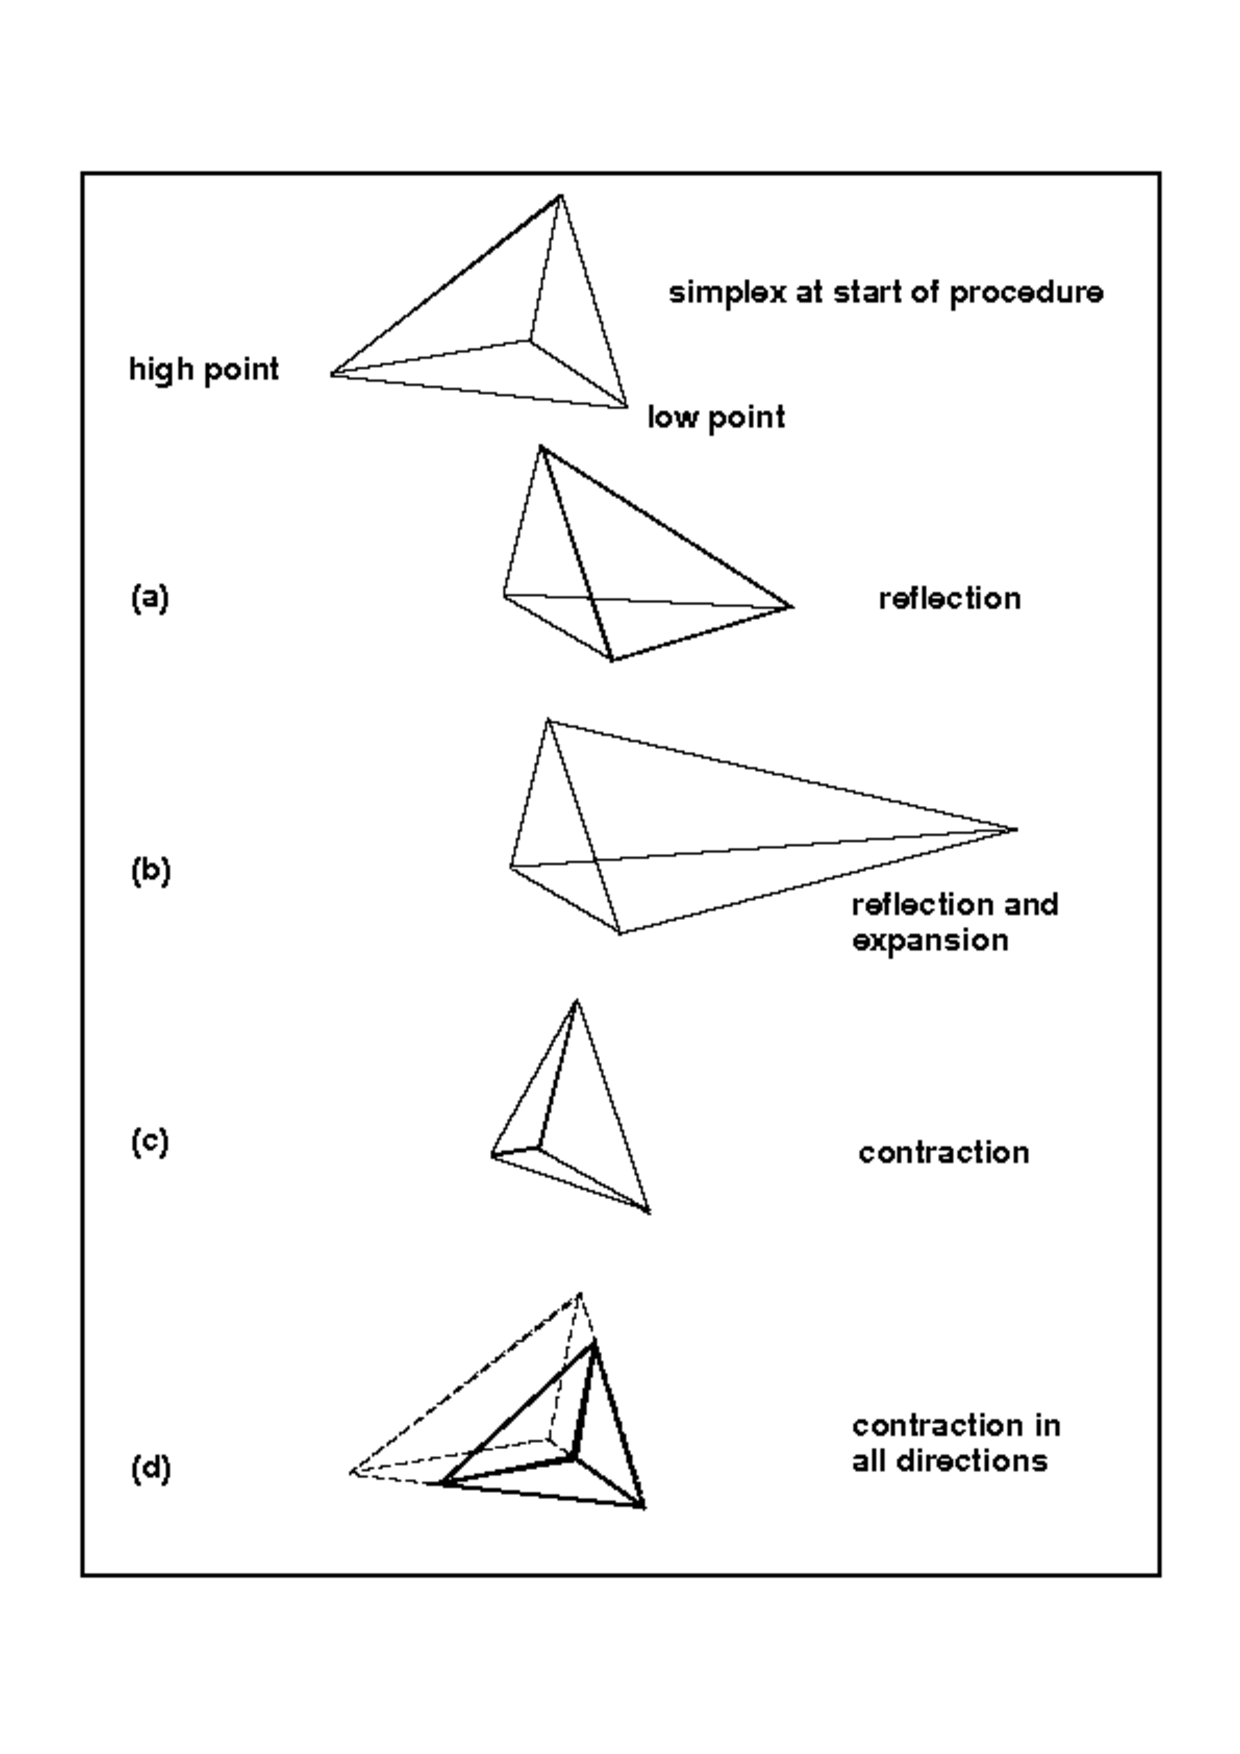
\includegraphics{image/neldermead.pdf}}

  \vspace*{-4em}
  \hspace*{16em}{\tiny\url{http://www.kniaz.net/software/RosNM.aspx}}
\end{frame}

\section{シミュレーテッド・アニーリング}

\begin{frame}[t,fragile]{確率過程を用いた最適化}
  \begin{itemize}
    \setlength{\itemsep}{1em}
  \item 最急降下法 (steepest decent) {\footnotesize \href{https://github.com/todo-group/computer-experiments/blob/master/exercise/optimization/mc_steepest_descent_1d.c}{example-2-L4/mc\_steepest\_descent\_1d.c}}
    \begin{itemize}
    \item 初期状態をランダムに定める
    \item 配位を少しだけ変化させる
    \item エネルギー(コスト関数)が小さくなるなら採択、大きくなるなら棄却
    \item 状態が変化しなくなるまでくり返す %$\Rightarrow$ 絶対零度でのMetropolis法
    \item 問題点 : エネルギー極小状態にすぐに捕まってしまう
    \end{itemize}
  \item 徐冷法 (simulated annealing) {\footnotesize \href{https://github.com/todo-group/computer-experiments/blob/master/exercise/optimization/simulated_annealing_1d.c}{example-2-L4/simulated\_annealing\_1d.c}}
    \begin{itemize}
    \item いきなり温度を零にするのではなく少しずつ下げていく
    \item どれくらいゆっくり下げれば良いか? $
      T(t) \ge cN / \log(t+2)
      $
    \item 実際には適当なスケジューリングで温度を下げ、何回か繰り返して最も良い結果を採択
    \end{itemize}
  \end{itemize}
\end{frame}

\begin{frame}[t,fragile]{最急降下法とシミュレーテッド・アニーリング}
  \noindent\resizebox{0.45\textwidth}{!}{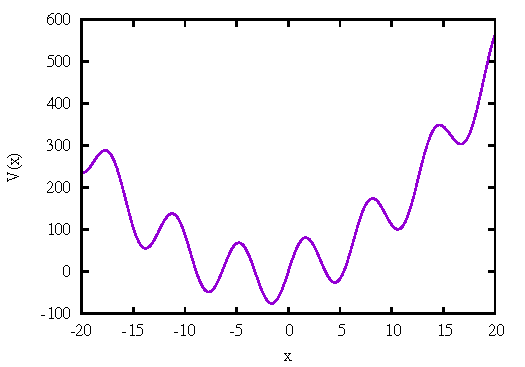
\includegraphics{image/potential.pdf}}

  \noindent\hspace*{.5em}\resizebox{0.43\textwidth}{!}{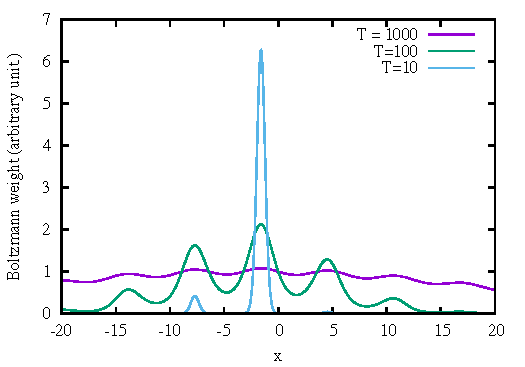
\includegraphics{image/boltzmann.pdf}}

  \vspace*{-17em}\hspace*{12.5em}\resizebox{0.6\textwidth}{!}{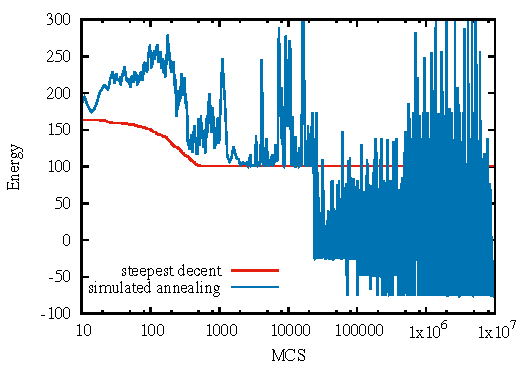
\includegraphics{image/energy.pdf}}

  \hspace*{17em}$T(t) = 100 - \frac{99}{10^7} t$
\end{frame}

\begin{frame}[t,fragile]{離散最適化問題への応用}
  \begin{itemize}
    \setlength{\itemsep}{1em}
  \item 微分を必要としないので、離散最適化問題にも適用可
    \begin{itemize}
    \item 例: 巡回セールスマン問題、数独、ナップザック問題
    \end{itemize}
  \item いかに状態とエネルギーを定義するかが重要
    \begin{itemize}
    \item 例: $n \times n$魔法陣 (行・列・ななめの和$M = n(n^2+1)/2$)
    \item 「状態」C: $1\sim n^2$の自然数をある順序でます目に並べたもの
    \item 「エネルギー」
      \[
      E(C) = \sum_{\rm row} (S_r-M)^2 + \sum_{\rm col} (S_c-M)^2 + \sum_{\rm diag} (S_d-M)^2
      \]
    \item 「正しい」魔方陣: $E(C) = 0$
    \end{itemize}
  \item 解の数(絶対零度のエントロピー)を求めるのにも利用できる
  \end{itemize}
\end{frame}


\section{}

\begin{frame}[t,fragile]{実習・講義予定}
  \begin{itemize}
    \setlength{\itemsep}{1em}
  \item 実習 EX5
    \begin{itemize}
    \item 特異値分解
    \item 線形回帰
    \end{itemize}
  \item 講義 L7
  \item 実習 EX6
  \end{itemize}
\end{frame}

\end{document}
